\section{Synchronization and Deadlocks}

\paragraph{Producer-Consumer Problem}
\begin{itemize}
  \item \textbf{Definition}:
  \begin{itemize}
    \item buffer is shared between producer and consumer (LIFO)
    \item \code{count} integer keeps track of number of currently available items
    \item producer produces item $ \to $ placed in buffer, \code{count++}
    \item buffer full $ \to $ producer needs to sleep until consumer consumed an item
    \item consumer consumes item $ \to $ remove item from buffer, \code{count--}
    \item buffer empty $ \to $ consumer needs to sleep until producer produces item
  \end{itemize}
  \item \textbf{Problem}: \emph{race condition} on \code{count}
\end{itemize}

\paragraph{Producer-Consumer Problem --- condition variables}
\begin{itemize}
  \item \textbf{Solution}: can be solved with mutex + 2 counting semaphores
  \begin{itemize}
    \item hard to understand
    \item hard to get right
    \item hard to transfer to other problems
  \end{itemize}
  \item \textbf{condition variables}: allow blocking until condition is met
  \begin{itemize}
    \item usually suitable for same problems but much easier to get right
  \end{itemize}
  \item \textbf{Idea}:
  \begin{itemize}
    \item new operation performs \emph{unlock}, \emph{sleep}, \emph{lock} atomically
    \item new wake-up operation is called with lock held
    \item[$ \to $] simple mutex lock/unlock around CS + no signal loss
  \end{itemize}
  \item \textbf{Pthread} condition variables:
  \begin{itemize}
    \item \code{pthread_cond_init}: create + initialize new CV
    \item \code{pthread_cond_destroy}: destroy + free existing CV
    \item \code{pthread_cond_wait}: block waiting for signal
    \item \code{pthread_cond_timedwait}: block waiting for signal or timer
    \item \code{pthread_cond_signal} : signal another thread to wake up
    \item \code{pthread_cond_broadcast}: signal all threads to wake up
  \end{itemize}
\end{itemize}
\begin{figure}[h]\centering\label{ConditionVariables}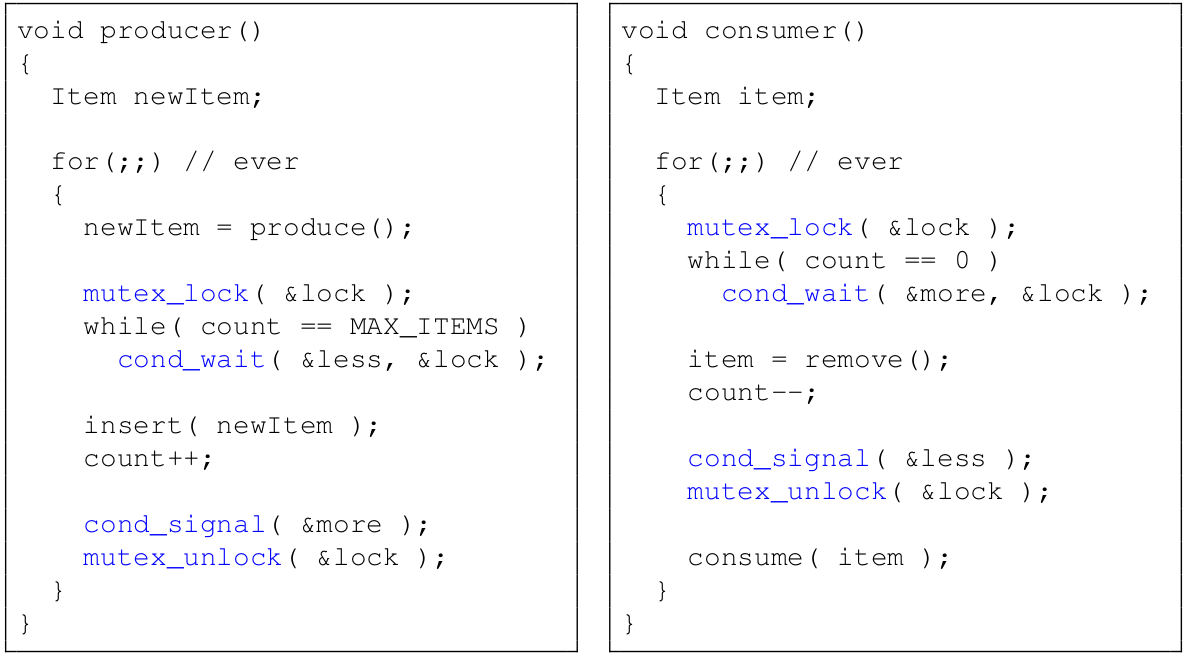
\includegraphics[width=0.33\textwidth]{ConditionVariables}\end{figure}

\paragraph{Reader-Writer Problem}
\begin{itemize}
  \item \textbf{Problem}: model access to shared data structures
  \begin{itemize}
    \item many threads compete to read/write same data
    \item \emph{readers}: only read data set, not performing any updates
    \item \emph{writers}: both read and write
    \item[$ \leadsto $] using single mutex for read/write operations is not a good solution! (unnecessarily blocking out multiple readers while no writer is present)
  \end{itemize}
  \item \textbf{Idea}: locking should reflect different semantics for reading/writing
  \begin{itemize}
    \item no writing thread $ \to $ multiple readers may be present
    \item writing thread $ \to $ no other reader/writer allowed
  \end{itemize}
\end{itemize}

\paragraph{Dining-Philosophers Problem}
\begin{itemize}
  \item \textbf{Definition}: 5 philosophers with cyclic workflow:
  \begin{enumerate}
    \item think
    \item get hungry
    \item grab one chopstick
    \item grab other chopstick
    \item put down chopsticks
  \end{enumerate}
  \item \textbf{Rules}:
  \begin{itemize}
    \item no communication
    \item no atomic grabbing of both chopsticks
    \item no wrestling
  \end{itemize}
  \item \textbf{Abstraction}: models threads competing for limited number of resources
  \textbf{Problem}: what happens if all philosophers grab left chopstick at once?
  \item \textbf{Deadlock workarounds}:
  \begin{itemize}
    \item \emph{deadlock avoidance}: just 4 philosophers allowed at table of 5
    \item \emph{deadlock prevention}: odd philosophers take left chopstick first, even ones take right first $ \to $ \emph{deadlock prevention}
  \end{itemize}
\end{itemize}
\begin{figure}[h]\centering\label{DiningPhilosophers}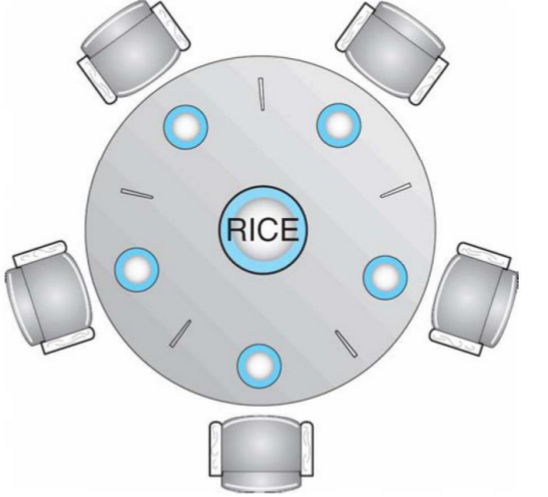
\includegraphics[width=0.2\textwidth]{DiningPhilosophers}\end{figure}

\paragraph{Deadlocks}
\begin{itemize}
  \item \textbf{Deadlocks} can arise if all four conditions hold simultaneously:
  \begin{itemize}
    \item \emph{mutual exclusion}: limited resource access (can only be shared with finite number of users)
    \item \emph{hold and wait}: wait for next resource while already holding at least one
    \item \emph{no preemption}: granted resource cannot be taken away but only handled back voluntarily
    \item \emph{circular wait}: possibility of circularity in requests graph
  \end{itemize}
\end{itemize}

\paragraph{Deadlocks --- countermeasures}
\begin{itemize}
  \item \textbf{prevention}: pro-active, make deadlocks impossible to occur
  \item \textbf{avoidance}: decide on allowed actions based on a-priori knowledge
  \item \textbf{detection} (\emph{recovery}): react after deadlock happened
\end{itemize}

\paragraph{Deadlocks --- prevention}
\begin{itemize}
  \item \textbf{Goal}: negate at least one of the required deadlock conditions:
  \begin{itemize}
    \item \emph{mutual exclusion}: buy more resources, split into pieces, virtualize
    \item \emph{hold and wait}: get all resources en-bloque, 2-phase-locking
    \item \emph{no preemption}: virtualize to make preemptable
    \item \emph{circular wait}: reorder resources, prevent through partial order on resources
  \end{itemize}
\end{itemize}

\paragraph{Deadlocks --- avoidance}
\begin{itemize}
  \item \textbf{safe state}: system is in safe state $ \to $ no deadlocks
  \item \textbf{unsafe state}: system is in unsafe state $ \to $ deadlocks possible
  \item \textbf{avoidance}: on every resource request decide if system stays in safe state
  \begin{itemize}
    \item[$ \to $] \emph{resource allocation graph}
  \end{itemize}
\end{itemize}

\paragraph{Deadlock Avoidance --- resource allocation graph}
\begin{itemize}
  \item \textbf{principle}: view system state as graph
  \begin{itemize}
    \item \emph{processes} = round nodes
    \item \emph{resources} = square nodes
    \item \emph{resource instance} = dot in resource node
    \item \emph{resource requests/assignments} = edges
    \begin{itemize}
      \item resource $ \to $ process = resource is assigned to process
      \item process $ \to $ resource = process is requesting resource
    \end{itemize}
  \end{itemize}
  \begin{figure}[h]\centering\label{ResourceAllocationGraph}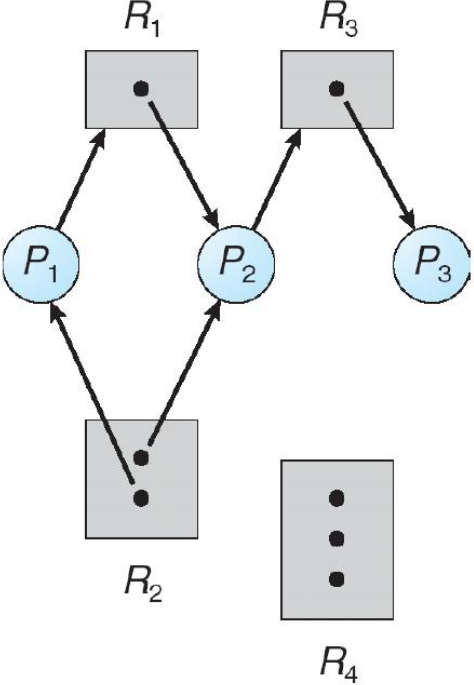
\includegraphics[width=0.12\textwidth]{ResourceAllocationGraph}\end{figure}
\end{itemize}

\paragraph{Deadlocks --- detection}
\begin{itemize}
  \item \textbf{Principle}: allow system to enter deadlock $ \to $ detection $ \to $ recovery scheme
  \item \textbf{wait-for graph} (WFG):
  \begin{itemize}
    \item \emph{processes} = nodes
    \item \emph{wait-for relationship} = edges
  \end{itemize}
  \item periodically invoke algorithm searching for cycle in graph
  \begin{itemize}
    \item[$ \leadsto $] cycle exists $ \to $ deadlock exists
  \end{itemize}
\end{itemize}
\begin{figure}[h]\centering\label{WaitForGraph}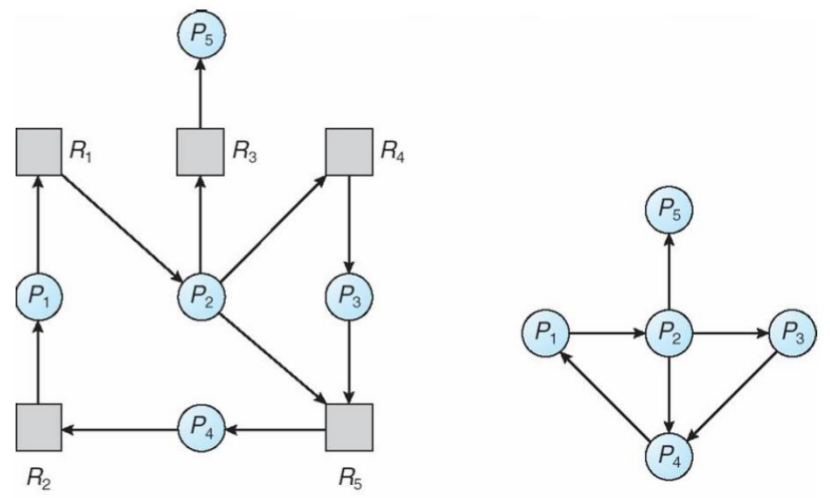
\includegraphics[width=0.33\textwidth]{WaitForGraph}\end{figure}

\paragraph{Deadlocks --- recovery}
\begin{itemize}
  \item \textbf{Process termination}:
  \begin{itemize}
    \item \emph{all}: abort all deadlocked processes
    \item \emph{selective}: abort one process at a time until deadlock is eliminated
  \end{itemize}
  \item \textbf{Termination order}: in which order should processes be aborted?
  \begin{itemize}
    \item process priority
    \item how long already computed? how much longer for completion?
    \item amount of resources used
    \item amount of resources needed for completion
    \item how many processes will need to be terminated
    \item interactive or batch?
  \end{itemize}
  \item \textbf{Resource preemption}:
  \begin{itemize}
    \item \emph{victim selection}: minimize cost
    \item \emph{rollback}: perform periodic snapshots, abort process to preempt resources $ \to $ restart from last safe state
    \item \emph{starvation}: same process may always be picked as victim $ \leadsto $ include rollback count in cost factor
  \end{itemize}
\end{itemize}

\begin{summary}
  \begin{itemize}
    \item \textbf{classical synchronization problems}: model synchronization problems occurring in reality
    \begin{itemize}
      \item \emph{producer-consumer}: shared use of buffers/queues
      \item \emph{reader-writer}: shared access to data structures
      \item \emph{dining philosophers}: competition for limited resources
    \end{itemize}
    \item such synchronization problems occur very often when programming operating systems
    \item \textbf{parallelism}: introduced by multiple processors + multiprogramming, needs to be considered carefully when writing OS
  \end{itemize}
\end{summary}